%----------------------------------------------------------------------------------------
%
% LaTeX-template for degree projects at LNU, Department of Mathematics
%
% Based on a template for degree projects in Computer Science, by Johan Hagelbäck
%
%----------------------------------------------------------------------------------------

%----------------------------------------------------------------------------------------
%	Settings and configuration
%----------------------------------------------------------------------------------------

\documentclass[a4paper,12pt]{article}

\usepackage[T1]{fontenc}
\usepackage[english]{babel}
\usepackage[utf8]{inputenc}
\usepackage{dtklogos}
\usepackage{wallpaper}
\usepackage[absolute]{textpos}
\usepackage[top=2cm, bottom=2.5cm, left=3cm, right=3cm]{geometry}
\usepackage{appendix}
\usepackage[nottoc]{tocbibind}
\usepackage[colorlinks=true,
            linkcolor=black,
            urlcolor=blue,
            citecolor=black]{hyperref}

\setcounter{secnumdepth}{3}
\setcounter{tocdepth}{3}

\usepackage{sectsty}
\sectionfont{\fontsize{14}{15}\selectfont}
\subsectionfont{\fontsize{12}{15}\selectfont}
\subsubsectionfont{\fontsize{12}{15}\selectfont}

\usepackage{csquotes} % Used to handle citations

\renewcommand{\thetable}{\arabic{section}.\arabic{table}}
\renewcommand{\thefigure}{\arabic{section}.\arabic{figure}}

%----------------------------------------------------------------------------------------
%	
%----------------------------------------------------------------------------------------
\newsavebox{\mybox}
\newlength{\mydepth}
\newlength{\myheight}

\newenvironment{sidebar}%
{\begin{lrbox}{\mybox}\begin{minipage}{\textwidth}}%
{\end{minipage}\end{lrbox}%
 \settodepth{\mydepth}{\usebox{\mybox}}%
 \settoheight{\myheight}{\usebox{\mybox}}%
 \addtolength{\myheight}{\mydepth}%
 \noindent\makebox[0pt]{\hspace{-20pt}\rule[-\mydepth]{1pt}{\myheight}}%
 \usebox{\mybox}}

%----------------------------------------------------------------------------------------
%	Title section
%----------------------------------------------------------------------------------------
\newcommand\BackgroundPic{
    \put(-2,-3){
    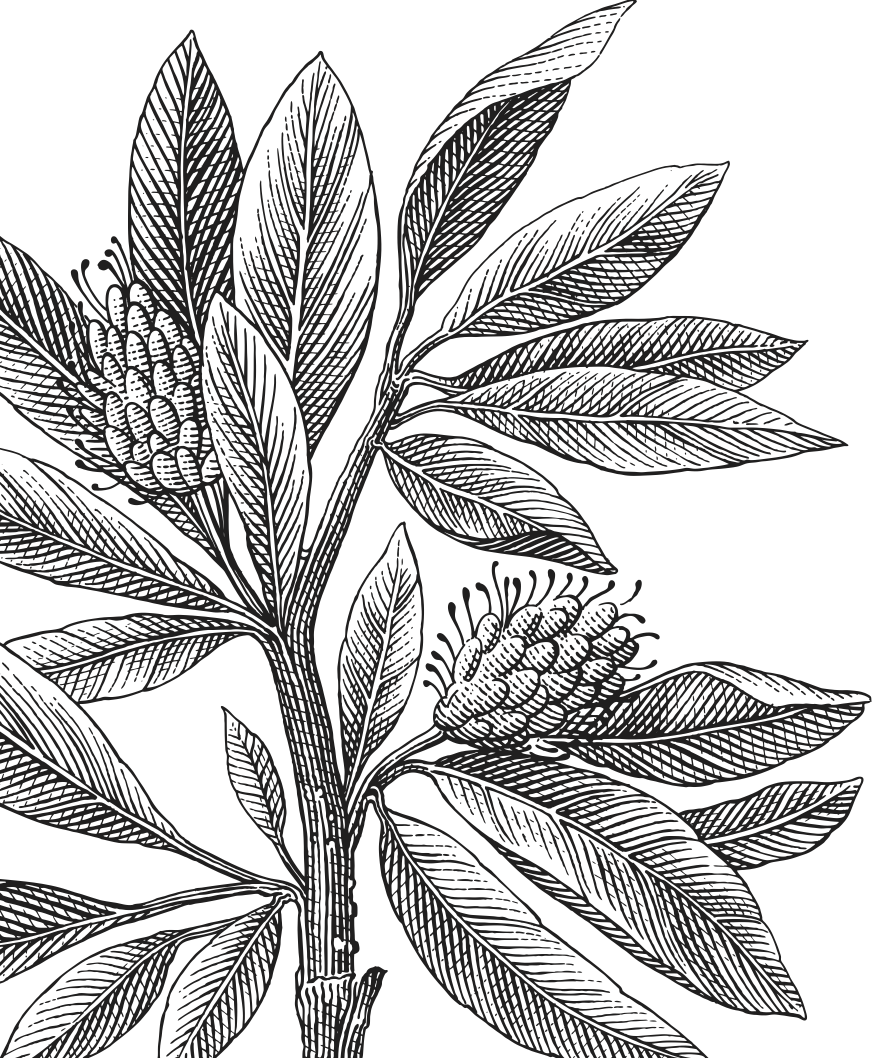
\includegraphics[keepaspectratio,scale=0.3]{lnu_etch.png} % Background picture
    }
}
\newcommand\BackgroundPicLogo{
    \put(30,740){
    
\includegraphics[keepaspectratio,scale=0.10]{logo.png} % Logo in upper left corner
    }
}

\title{	
\vspace{-8cm}
\begin{sidebar}
    \vspace{10cm}
    \normalfont \normalsize
    \Huge \sf Bachelor Thesis \\
    \vspace{-1.3cm}
\end{sidebar}
\vspace{3cm}
\begin{flushleft}
    \huge \bf Optimizing Queueing Performance in Distributed Systems\\
    \it \LARGE - A Queueing Theory Approach with RabbitMQ
\end{flushleft}
\null
\vfill
\begin{textblock}{6}(10,13)
\begin{flushright}
\begin{minipage}{\textwidth}
\begin{flushleft} \normalsize
\emph{Author:} Andreas Lymalm\\
\emph{Supervisor:} Andreas Petersson\\
\emph{Examiner:} Roger Pettersson\\ 
\emph{Semester:} Spring 2025 \\ %
\emph{Subject:} Mathematics (2MA41E) \\ % Subject area
\end{flushleft}
\end{minipage}
\end{flushright}
\end{textblock}
}

\date{}

\begin{document}
\pagenumbering{gobble}
\newgeometry{left=5cm}
\AddToShipoutPicture*{\BackgroundPic}
\AddToShipoutPicture*{\BackgroundPicLogo}
\maketitle
\restoregeometry
\clearpage
%----------------------------------------------------------------------------------------
%	Abstract
%----------------------------------------------------------------------------------------
\selectlanguage{english}
\begin{abstract}

\end{abstract}

\newpage
%----------------------------------------------------------------------------------------
%	Acknowledgements
%----------------------------------------------------------------------------------------

\section*{Acknowledgements}


%----------------------------------------------------------------------------------------
\newpage
\pagenumbering{gobble}
\tableofcontents % Table of contents
\newpage
\pagenumbering{arabic}

%----------------------------------------------------------------------------------------
%
%	Here follows the actual text contents of the report.
%
%----------------------------------------------------------------------------------------

\section{Introduction}

\section{Theoretical Background}

    \subsection{Queueing Theory}
    Queueing theory is the mathematical study of queues, which can be applied, e.g., in systems like computer networks, manufacturing, and service systems. It provides a framework for analyzing how \textit{entities} (such as messages, tasks, or customers) arrive, wait, and are served in a system. 

        \subsubsection{Characteristics}
        The main characteristics of queueing systems include arrival patterns, service patterns, queue disciplines, system capacity, number of servers, and number of service stages \cite{shortle2018}.
        
        \textit{Arrival patterns} defines how entities arrive in the system. For example, in transportation systems it could be a scheduled arrival process, but in many systems a so called \textit{Poisson arrival process} is often used, which models random independent arrivals.

        \textit{Service patterns} defines how entities are processed, with respect to service times, in the system. Some examples are exponential service times for e.g. call centers and deterministic processing times in e.g. manufacturing systems. 

        \textit{Queue disciplines} defines server order rules of the system, such as First-Come-First-Served (FCFS), Last-Come-First-Served (LCFS), and priority queues used in emergency services.

        \textit{System capacity} defines the limits on the number of entities a system can handle. Examples include finite queue lengths in computer buffers and unlimited queue sizes in cloud-based message systems.

        \textit{Number of servers} defines the number of servers in the system. For example, an ATM is a single-server system, while the cashiers in the supermarket are part of a multiple-server system. 

        \textit{Number of service stages} defines the number of steps in the system. A several-step system could be a drive-through in a fast food restaurant, where customers order, pay, and finally receive their food. 

        \subsubsection{Queueing Models}
        To mathematically analyze the performance of a queueing system, there are, with respect to the main characteristics, some common models that are used, and that will be of special interest for this thesis. Specifically, these systems are focusing on the arrival pattern, service pattern, and the number of systems \cite{shortle2018}. 

        The \textit{M/M/1} queue model is a single-server queue system (represented by the \textit{1}), where arrivals follow a Poisson arrival process (represented by the first \textit{M}) and service times are exponentially distributed (represented by the second \textit{M}). 
        
        The \textit{M/M/c} queue model is the same as the former model, but features multiple servers (represented by the \textit{c}).
        
        The \textit{M/G/1} queue model is a single-server system with a Poisson arrival process, like the first model, but which service times follows a general arbitrary distribution (represented by the \textit{G}).
    
    \subsection{Traffic Modeling}
    Traffic modeling builds on queue arrival patterns, focusing on varying demand impacting arrivals. These are the models of interest \cite{ross2022}.

    A \textit{Poisson Arrival Process}, as described in the characteristics chapter, assumes that entities arrive randomly and independently over time and is widely used for modeling network systems.

    \textit{Bursty Traffic} 

    \textit{Periodic Traffic}

    \textit{Traffic Load Variation}

    \textit{Network Congestion Effects}

\section{Methods}

    \subsection{Mathematical Modeling}
    
    \subsection{Simulation Setup}
    
    \subsection{Experimental Setup}

\section{Results}

    \subsection{Simulation Results}

    \subsection{Experimental Results}

    \subsection{Comparison}

\section{Discussion}

%----------------------------------------------------------------------------------------
%	List of References
%-----------------------------------------------------------------------------------------


\hypersetup{urlcolor=black}
\bibliographystyle{IEEEtran}
\bibliography{references}
\newpage

%----------------------------------------------------------------------------------------
%	Appendices
%-----------------------------------------------------------------------------------------

\appendix

\section{Appendix 1}


\end{document}
